\documentclass[12pt,a4paper]{article}

\usepackage[utf8]{inputenc}
\usepackage[T1]{fontenc}
\usepackage[french]{babel}

\usepackage{geometry}
\geometry{
    top=1.5cm,
    bottom=1.5cm,
    left=1.6cm,
    right=1.6cm
}

\usepackage{graphicx}
\usepackage{booktabs}
\usepackage{amsmath}
\usepackage{hyperref}

% Réduction des espaces
\setlength{\parindent}{0pt}
\setlength{\parskip}{3pt}

\usepackage{titlesec}
\titlespacing*{\section}{0pt}{6pt}{3pt}
\titlespacing*{\subsection}{0pt}{4pt}{2pt}

% Page de titre
\title{
    \vspace{-1cm}

    \includegraphics[width=0.25\textwidth]{logopariscité.png}\\[0.3cm]

    
\includegraphics[height=1.5cm]{module.png}

    \vspace{0.5cm}

    \textbf{Détection de masques faciaux par Faster R-CNN}
}

\author{
    \textbf{Étudiant :} Fallou Diouf\\[0.2cm]
    \textbf{Professeur :} Pr Sylvain Lobry
}

\date{}

\begin{document}

\maketitle

\vspace{-0.5cm}
\section{Introduction}

Ce travail porte sur la détection automatique du port du masque facial
à partir d'images. Le jeu de données contient trois classes :
\texttt{with\_mask}, \texttt{without\_mask} et
\texttt{mask\_weared\_incorrect}. Les annotations sont fournies sous
forme de fichiers XML contenant les classes et les coordonnées des
boîtes englobantes. Un modèle Faster R-CNN pré-entraîné sur COCO est
adapté à cette tâche.

\section{Données et annotations}

Le jeu de données contient 853 images et 853 fichiers XML.

\textbf{Réponse 1 -- Structure des annotations.}
Chaque fichier XML contient les objets présents dans l'image, leur nom
de classe et leur boîte englobante. Les coordonnées sont données sous
la forme $[x_{\min},y_{\min},x_{\max},y_{\max}]$, avec
$(x_{\min},y_{\min})$ en haut à gauche et
$(x_{\max},y_{\max})$ en bas à droite. Par exemple,
\texttt{maksssksksss0.xml} contient trois objets avec les boîtes
$[79,105,109,142]$, $[185,100,226,144]$ et
$[325,90,360,141]$.

\textbf{Réponse 2 -- Sources de biais.}
Plusieurs biais potentiels peuvent être présents : déséquilibre entre
les classes, différences de luminosité et de qualité d'image,
arrière-plans variés, tailles et orientations différentes des visages.
Le modèle peut ainsi apprendre certaines caractéristiques propres au
jeu de données en plus des caractéristiques liées au masque.

\section{Préparation des données}

\textbf{Réponse 3 -- Découpage du jeu de données.}
Les 853 images ont été divisées aléatoirement en 511 images
d'entraînement, 171 de validation et 171 de test, soit environ
60\,\%, 20\,\% et 20\,\%. Pour un jeu de données de cette taille,
l'augmentation des données, la validation croisée et le transfert
d'apprentissage constituent des stratégies permettant d'améliorer la
généralisation.

\textbf{Réponse 4 -- Répartition des classes.}
Le comptage des objets annotés donne :

\begin{center}
\begin{tabular}{l r}
\toprule
Classe & Nombre \\
\midrule
\texttt{with\_mask} & 3232 \\
\texttt{without\_mask} & 717 \\
\texttt{mask\_weared\_incorrect} & 123 \\
\midrule
Total & 4072 \\
\bottomrule
\end{tabular}
\end{center}

La classe \texttt{with\_mask} représente 79.4\,\% des objets,
\texttt{without\_mask} 17.6\,\% et
\texttt{mask\_weared\_incorrect} seulement 3.0\,\%. Le jeu de données
est donc fortement déséquilibré.

\section{Modèle et entraînement}

Le modèle utilisé est un Faster R-CNN avec un backbone ResNet-50 et une
Feature Pyramid Network (FPN), pré-entraîné sur COCO. Sa tête de
classification a été remplacée pour produire quatre classes : les
trois classes du problème et la classe \textit{background}. Les images
sont converties en tenseurs et les annotations sont fournies sous forme
de boîtes et d'indices de classes. Une fonction \textit{collate}
permet de gérer le nombre variable d'objets par image.

\textbf{Réponse 5 -- Hyperparamètres.}
L'entraînement utilise SGD avec un taux d'apprentissage de $0.001$,
un momentum de $0.01$, une taille de batch de 2 et 5 époques. Ces
valeurs constituent des paramètres initiaux d'expérimentation et n'ont
pas été obtenues par une recherche systématique.

\section{Résultats et analyse}

La figure~\ref{fig:loss} montre l'évolution des losses. La loss
d'entraînement diminue de 0.3199 à 0.1761 et la loss de validation de
0.3017 à 0.2072. Les deux courbes diminuent pendant les cinq époques :
aucune remontée de la validation loss n'est observée, ce qui ne permet
pas de conclure à un surapprentissage à partir de ces seules courbes.

\begin{figure}[h]
\centering
\includegraphics[width=0.72\linewidth]{/Users/falloudiouf/Desktop/DeepLearningForVision/TP3_Objects_Detection/FaceMaskDetection/outputs/figures/loss_curve.png}
\caption{Évolution des losses d'entraînement et de validation.}
\label{fig:loss}
\end{figure}

Sur l'ensemble de test, composé de 171 images, la loss est de 0.1860.
Les prédictions sont évaluées avec un seuil de confiance de 0.5 et un
seuil d'IoU de 0.5 pour la correspondance entre boîtes prédites et
annotations.

\begin{center}
\begin{tabular}{l c c c}
\toprule
Classe & Precision & Recall & F1 \\
\midrule
\texttt{with\_mask} & 0.8013 & 0.8386 & 0.8195 \\
\texttt{without\_mask} & 0.6824 & 0.3671 & 0.4774 \\
\texttt{mask\_weared\_incorrect} & 0.0000 & 0.0000 & 0.0000 \\
\midrule
Global & 0.7894 & 0.7317 & 0.7595 \\
\bottomrule
\end{tabular}
\end{center}

Les performances varient fortement selon les classes. La classe
\texttt{with\_mask}, majoritaire, obtient un F1-score de 0.8195.
Le rappel de \texttt{without\_mask} est plus faible (0.3671).
La classe \texttt{mask\_weared\_incorrect} n'est correctement détectée
dans aucun cas de l'évaluation. Ce résultat est cohérent avec son très
faible nombre d'exemples : seulement 123 objets contre 3232 pour
\texttt{with\_mask}. Les visualisations montrent également des
prédictions correctes sur plusieurs visages ainsi que des confusions,
notamment entre \texttt{with\_mask} et les autres classes.

\section{Conclusion}

Ce travail a permis de mettre en place une chaîne complète de détection
d'objets, depuis l'exploitation des annotations XML jusqu'à
l'évaluation d'un Faster R-CNN. L'entraînement pendant cinq époques
réduit les losses d'entraînement et de validation. Sur le test, le
modèle obtient une précision globale de 0.7894, un rappel de 0.7317 et
un F1-score de 0.7595. Les résultats montrent toutefois l'impact du
déséquilibre des classes, particulièrement pour
\texttt{mask\_weared\_incorrect}. Des données supplémentaires pour les
classes minoritaires, de l'augmentation de données et une recherche
d'hyperparamètres pourraient être étudiées pour améliorer les
performances.

\subsection{Analyse qualitative}

Les visualisations permettent de comparer les annotations réelles
(\textit{Ground Truth}) aux prédictions du modèle. Plusieurs visages
sont correctement localisés et classifiés, notamment pour la classe
\texttt{with\_mask}. Les scores de confiance sont généralement élevés
pour ces détections.

Cependant, certaines erreurs sont observées. Le modèle confond
notamment certaines personnes sans masque avec la classe
\texttt{with\_mask}. La classe \texttt{mask\_weared\_incorrect} constitue
la principale difficulté, ce qui est cohérent avec son faible nombre
d'exemples dans le jeu de données.

\begin{figure}[h]
\centering
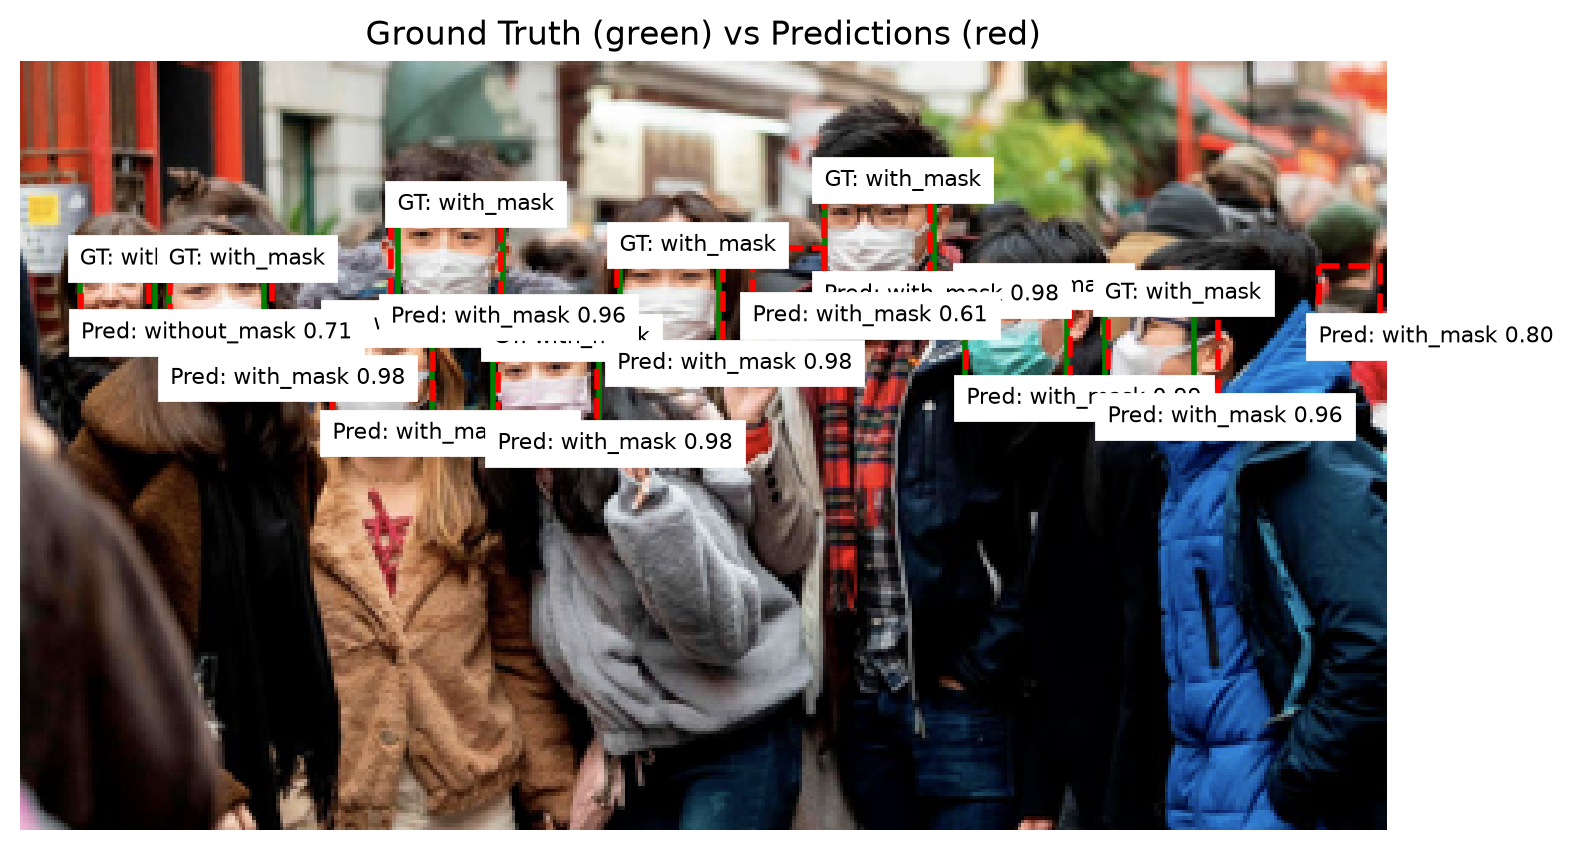
\includegraphics[width=0.48\linewidth]{../outputs/figures/prediction_0.png}
\hfill
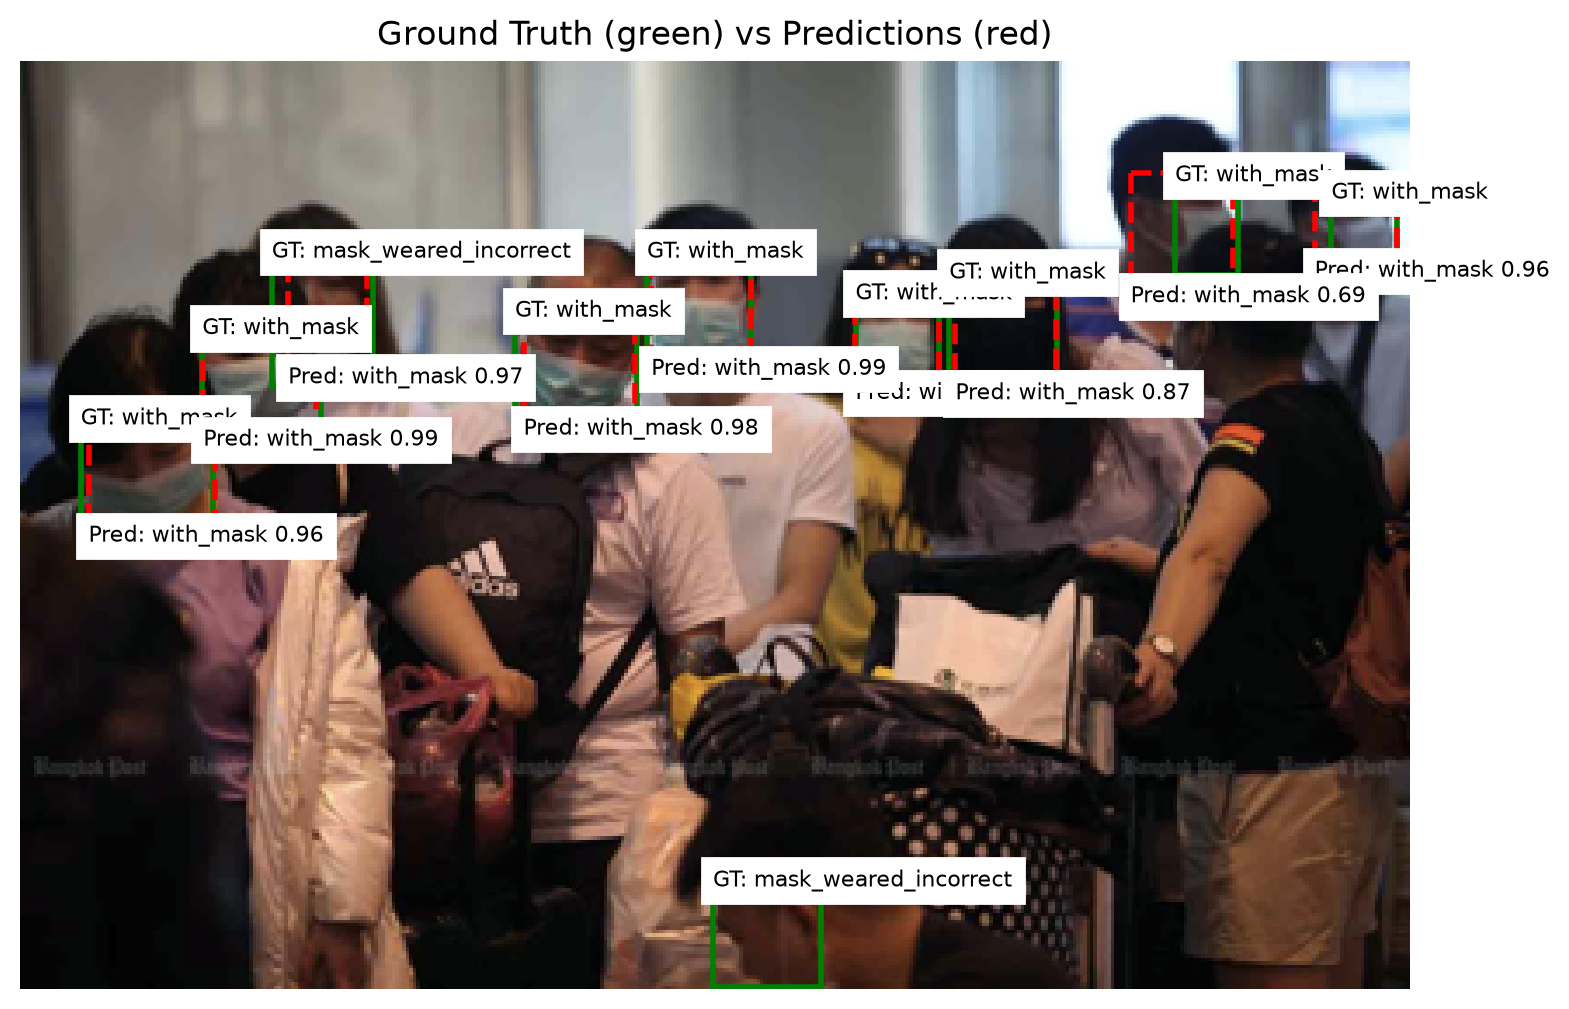
\includegraphics[width=0.48\linewidth]{../outputs/figures/prediction_4.png}
\caption{Exemples de prédictions du modèle : annotations réelles en
vert et prédictions en rouge.}
\label{fig:predictions}
\end{figure}

\end{document}